%OLD
\section{Workflow of Running a WE Simulation}

An overview of the workflow for running a WE simulation using WESTPA is detailed below. 
This workflow is only meant to give a sense of the mechanics and flow of using WESTPA once your system and WE parameters have already been carefully chosen. See \textbf{Table \ref{intro:table2}} for a summary of all files mentioned in this workflow.

\begin{table}
\caption{WEST\_SIM\_ROOT organization and file explanations}
\label{intro:table2}
\centering
\begin{tabular}{| r | l |}
\hline
\verb|bstates/| & directory containing basis states \\
\hline
\verb|env.sh| & set environment variables \\
\hline
\verb|init.sh| & initialize the WESTPA simulation \\
\hline
\verb|common_files/| & directory containing files for \\
{} & dynamics (i.e. topologies) \\
\hline
\verb|run.sh| & run the WESTPA simulation \\
\hline
\verb|tstate.file| & define the target state (for steady state \\
{} & simulations only) \\
\hline
\verb|west.cfg| & specify main WE simulation parameters \\
\hline
\verb|westpa_scripts/| & directory containing essential scripts \\
\hline
\verb|system.py| & a separate script to define functions or \\
{} & parameters (optional) \\
\hline
\verb|reference/| & directory containing reference files for \\
{} & calculations (optional) \\
\hline
\end{tabular}
\end{table}

\noindent\textbf{Overall Flow}

\textbf{Ready:} The purpose of this step is to ensure that the chosen WE parameters are correctly specified in the proper places and that all environment variables are correctly set. 
Most of the WE parameters (such as the number of WE iterations, binning scheme etc.) and auxiliary datasets (auxdata; see \textbf{Section \ref{tut:p53-int}}) are specified in the \verb|west.cfg| file. 
You can view an example of this file in any of the tutorials below; labels exist directing where to specify each parameter. 
More complex binning schemes (such as recursive schemes or schemes involving functional bin mappers) can be specified in an external file called \verb|system.py|. 
A user may also choose to write functions to this file. 
Usually, these functions will calculate progress coordinate or auxiliary data and are more complex than usual.

The environment is set up in the \verb|env.sh| file. 
The location of the main WESTPA simulation directory (\verb|$WEST_SIM_ROOT|) and the location of dynamics/analysis programs are placed in your system path. 
When setting up WESTPA on a cluster, program modules will be loaded in the \verb|runwe.slurm| file instead of the \verb|env.sh| file (see \textbf{Section \ref{tut:basic-nacl-3}} and view the cluster-specific \verb|runwe.slurm| file). 
It is a best practice to define variables in \verb|env.sh| for each program that will be called. 
These variables should contain the full path to that program (such as \verb|CPPTRAJ=$(which cpptraj|), see \textbf{Section \ref{intro:minimizing_traffic}} for more information). 
Always source \verb|env.sh| before trying to run WESTPA just to see if any errors appear relating to programs not being found. 
If errors are present, edit \verb|env.sh| to specify the proper locations of programs and try to source it again. 
The goal of this action is to make sure that any issues with your environment are fixed before continuing so that troubleshooting becomes much easier later on. 

\textbf{Set:} After setting up the system environment and specifying the WE parameters, users will need to initialize the simulation. 
This involves running the \verb|init.sh| script, which will take an initial structure (or structures), calculate a progress coordinate (pcoord for short, this is also the name used in WESTPA datasets pertaining to the progress coordinate) value for that structure and then place that structure in the appropriate bin. 
The \verb|init.sh| file is also the location where users can specify whether the simulation will be run under equilibrium or steady-state conditions. 

Place the starting structure(s) in the \verb|bstates/| directory. 
The structure should be a coordinate file giving the starting configuration of your system (e.g. Amber restart file). 
The \verb|bstate.file| tells WESTPA which structure to use as the initial structure for the simulation. 
If you have only one structure, this file will contain the name of that structure only; if you have more than one structure, \verb|bstate.file| should list each structure along with its associated statistical weight. 
An example of the latter is a representative ensemble of unbound protein conformations in a binding process that could be generated using a prior equilibrium WE simulation \citep{Zwier2016,Saglam2019}. 

Next, specify whether the simulation will be run under equilibrium or steady-state conditions. 
This specification is made in the \verb|init.sh| file. 
Including a \verb|TSTATE_ARGS| argument for \verb|w_init| will signal for WESTPA to run under steady state conditions. 
The \verb|tstate.txt| file in the main simulation directory is where the progress coordinate value of the target state is specified. 
If the \verb|TSTATE_ARGS| argument is absent, the simulation will be run under equilibrium conditions. 
See the tutorials in \textbf{Sections \ref{tut:nacl-basic} and \ref{tut:p53-int}} below for examples of how \verb|init.sh| will change from running a steady-state simulation versus an equilibrium simulation (respectively).

Running \verb|init.sh| will cause WESTPA to execute \verb|get_pcoord.sh|, which is a script located in \verb|westpa_scripts/|. 
This script will give an initial progress-coordinate value for the basis state(s) (located in \verb|bstates/|) to WESTPA.


Users will need to modify \verb|get_pcoord.sh| to either read or calculate the progress coordinate for their particular simulation.
For instance, in the \textbf{Basic Tutorial \ref{tut:nacl-basic}}, the distance between the Na\textsuperscript{+} and Cl\textsuperscript{-} ions is used as the progress coordinate.
The \verb|get_pcoord.sh| file for that tutorial simply prints the contents of an already-existing file (\verb|pcoord.init|, which already contains the calculated value) and passes that value to WESTPA. 
However, \verb|get_pcoord.sh| can also perform the calculation for the basis state, as in the \textbf{Intermediate Tutorial \ref{tut:p53-int}}.
However this is done, a value (or values) for that progress coordinate should be echoed into \verb|WEST_PCOORD_RETURN|, a WESTPA variable containing all of the progress coordinate values for the entire simulation (see \textbf{Section \ref{tut:p53-int}} for the added considerations if a two-dimensional progress coordinate is used).

If errors appear while trying to initialize the simulation, the following troubleshooting methods are recommended. 
First, make sure that the command entered in \verb|get_pcoord.sh| properly calculates the progress coordinate. 
Copy the initial structure from the \verb|bstates/| directory to another directory and run the command. 
If the command does not work, make sure the proper atoms and residues are selected and then try running the command again. 
If the command works, make sure that the calculated value is being successfully echoed into \verb|WEST_PCOORD_RETURN|.

To make troubleshooting easier, turn on logging for the \verb|get_pcoord| step in the \verb|west.cfg| file. 
By setting the location of the standard output (stdout) and/or standard error (stderr) to \verb|$WEST_SIM_ROOT/get_pcoord.log|, you can more closely monitor the output of the \verb|get_pcoord.sh| script to try to find out where things are not working.

\textbf{Go:} Running the \verb|run.sh| script will start a WESTPA simulation. 
If \verb|init.sh| was just run, a new simulation will begin and continue until the number of WE iterations specified in \verb|west.cfg| have been completed. 
If the simulation was stopped after previously running, \verb|run.sh| will continue the simulation from the point at which it was stopped. 
If WESTPA is being run on a cluster, then this script will take the form of a Slurm or other submission script (such as \verb|runwe.slurm|, see the \textbf{Basic Tutorial \ref{tut:nacl-basic}} for an example). 
WESTPA will propagate dynamics for one trajectory segment (of length $\tau$) and calculate progress coordinate values (and all auxiliary data) for the propagated structure(s). 
After completing a trajectory segment, WESTPA will combine and replicate trajectories to maintain the target number of trajectories per bin (as specified in the \verb|west.cfg| file). 
One cycle of dynamics and combination/replication is referred to as a single WE iteration. 
The number of iterations is repeated until the observable of interest (e.g. rate constant) is reasonably converged.

Running \verb|run.sh| will cause WESTPA to execute \verb|runseg.sh|, which is a script similar to \verb|get_pcoord.sh|, located in \verb|westpa_scripts/|. 
Users will need to modify \verb|runseg.sh| to call the dynamics engine and calculate the appropriate progress coordinate (and auxiliary data) value(s). 
Refer to the \verb|runseg.sh| file in the \textbf{Basic Tutorial \ref{tut:nacl-basic}} as an example. 
This particular simulation uses Amber’s \verb|pmemd| program for dynamics propagation. 
Running this program requires a certain input/output syntax that is specific to the dynamics engine (such as Gromacs or OpenMM). 
The section of this file that calculates the progress coordinate will be identical to that in the \verb|get_pcoord.sh| file. If a user is collecting auxiliary data (as specified in the \verb|west.cfg| file), those values will need to be calculated after calculating the progress coordinate value (see \textbf{Intermediate Tutorial \ref{tut:p53-int}}).

Since \verb|runseg.sh| will cause many different files to be generated, it is important to consider how WESTPA is handling these files, especially when using a shared file space such as on a cluster. 
The methods used in the example \verb|runseg.sh| files that have been provided in the tutorials below are sufficient in most cases, but please refer to \textbf{Section \ref{intro:minimizing_traffic}} for a discussion on file management and network traffic.

If there are any errors in the WESTPA setup (e.g. incorrect number of elements in the pcoord array, misplaced input files), the simulation will not proceed past the first WE iteration. 
If this is the case, check the \verb|west.log| file to see if there is a good reason for why the simulation is failing. 
Usually, however, detailed logging of any errors is available in the \verb|seg_logs/| directory for each segment of each iteration. 
View the segment log for a particular segment to see if the dynamics are completing successfully and that the progress coordinate (and auxdata) values are being calculated and passed to the appropriate variables (such as \verb|WEST_PCOORD_RETURN|).

If the dynamics fail to start, copy all necessary input files into an empty directory and run the dynamics manually. 
If no errors appear, make sure that your progress coordinate consists of the proper number of datapoints (as specified in the \verb|west.cfg| file). Also remember that you must include the parent coordinate file as your first data point when storing the progress coordinate data. This will ensure that the analysis tools work properly.

This is determined by the frequency at which the progress coordinate is being calculated. 
For example, if WESTPA expects 50 progress coordinate values per $\tau$ and only receives 10 values, the simulation will fail after the first WE iteration. 
Check the dynamics input file (\verb|md.in| in the \textbf{Basic and Intermediate tutorials \ref{tut:nacl-basic}-\ref{tut:p53-int}}) to make sure that the coordinates of your system are being saved at a frequency that matches the number of specified progress coordinate values.

If the simulation proceeds to the second iteration, there should not be any errors in the WESTPA setup. 
To monitor the progress of the WE simulation, use \verb|w_pdist| to generate probability distributions as a function of your progress coordinate and WE iteration. 
WESTPA’s \verb|plothist| command will allow you to visualize these probabity distributions with a few different visualization options (see \textbf{Basic and Intermediate Tutorials \ref{tut:nacl-basic}-\ref{tut:p53-int}}).

\textbf{Analyze:} All data generated from the simulation is contained in one place: the \verb|west.h5 file|. 
From this data, users can track the evolution of progress coordinate values, calculate fluxes into certain bins or states (see the \verb|w_ipa| analysis tutorial in \textbf{Section \ref{tut:analysis_adv_w_ipa}}) and view other statistics pertaining to the simulation. 
To visualize a completed trajectory, refer to \textbf{Basic Tutorial \ref{tut:nacl-basic}} and the \textbf{Analysis Tutorial \ref{tut:analysis-adv}}involving the visualization of trajectories(\textbf{Section \ref{tut:analysis_adv_visualization}}).

To assess the convergence of the simulation, a user might want to monitor the evolution of the flux into a target state as a function of the number of WE iterations by using the hdfview program to plot the \verb|target_flux_evolution| dataset in the \verb|direct.h5| file generated by \verb|w_ipa| (see \textbf{Basic Tutorial \ref{tut:nacl-basic}}). 

\section{Additional Simulation Workflow with WESTPA 2.0 Upgrades}

Given the major upgrades in the WESTPA 2.0 software package \citep{russo_westpa_2022}, we recommend the three-stage simulation workflow illustrated in \textbf{Figure \ref{fig:workflow}}. 
These workflow details are meant to supplement the simulation workflow outlined above. 
Details of the particular schemes mentioned are provided in the relevant \textbf{Advanced tutorials \ref{tut:binless}-\ref{tut:bng-adv}}.

In the first (“Ready”) stage, if one uses a binned resampling scheme, we recommend using one of the two adaptive binning schemes available in WESTPA 2.0: the minimal adaptive binning (MAB) scheme or adaptive Voronoi binning scheme.
These adaptive binning schemes enable quicker explorations of the chosen progress coordinate than manual, fixed binning schemes. 
The MAB scheme is effective at surmounting barriers in a direction of interest \citep{torrillo_minimal_2021} while the adaptive Voronoi binning scheme \citep{zhang_exact_2010} is ideal for enhanced sampling in high-dimensional space (more than three dimensions) when all parts of the progress-coordinate space are potentially important. 
However, if progress-coordinate space includes, for example, undesirable unfolded protein conformations, adaptive Voronoi binning might allocate bins and computing resources to those regions. 
Besides the adaptive binning schemes, one can opt for a “binless” resampling scheme by defining a grouping function as described in \textbf{Advanced Tutorial \ref{tut:binless}} below. 
The choice of $\tau$ (the resampling interval used for your WE simulation) should also be made on a system-by-system basis, with a sufficiently long time interval to capture relevant motions of interest but not so long that no net progress is made toward the target state. 
Examples of $\tau$ values used for various systems in previous WE studies are provided in the first suite of WESTPA tutorials \citep{bogetti_suite_2019}, but some trial-and-error will likely be necessary.
Convergence of a WE simulation will ultimately depend on the overall goal of running the simulation, but will most likely involve the time-evolution of an observable of interest leveling off over time (e.g., trajectory flux into a user-defined target state). 
If the convergence criterion is not met, a WE simulation using WESTPA can be resumed by simply running the \verb|run.sh| script or resubmitting the job if it was originally run with slurm. 
Even if changes were made to the progress coordinate or binning, WESTPA will incorporate those changes and resume the simulation accordingly.

In the second (“Set”) stage, we recommend starting the WE simulation from multiple, pre-equilibrated starting conformations that are representative of the initial stable state (at least one “basis state” for each trajectory walker) to improve the sampling of the initial state and diversity of generated pathways to the target state. 
Initial structures for a WE simulation should be chosen on a system-by-system basis, but in general, more starting structures (each with a slightly different initial configuration) should provide you with a more diverse trajectory ensemble. 
When the initial state of interest is well-defined, only a small number of structures may be necessary, but a truly heterogeneous initial state such as the unbound or unfolded states will require more structures to be representative of the intrinsic diversity.  
As discussed in \textbf{Section \ref{tut:binless}}, these "basis" structures will govern the recycling process (if used), so care should be exercised in choosing them.

In the third (“Go/Analyze”) stage, we recommend applying one of the following three options to further accelerate convergence to a steady state once successful pathways are generated. 
The Rates from Event Durations (RED) analysis scheme \citep{degrave_red_2021} estimates rate constants more efficiently than the original WE scheme \citep{huber_weighted-ensemble_1996} by exploiting information in the transient region of the simulation.
Another option is the haMSM plugin, which employs a fine-grained “microbin” analysis and can be used to not only estimate rate constants following WESTPA simulation (e.g., for the seconds-timescale coronavirus spike opening process \citep{casalino_ai-driven_2021}), but to also restart trajectories with their weights adjusted for a steady state \citep{russo_westpa_2022}. 
Because restarts in the haMSM plugin are initiated from configurations occurring throughout previously run trajectories, the continuity of the generated pathways is broken. 
The third option is the weighted ensemble steady state (WESS) plugin \citep{bhatt_steady-state_2010}, which uses the less fine-grained WE bins to estimate steady state but preserves the continuity of pathways, restarting from only the final points of trajectories. 
While all trajectory files of the chosen dynamics engine are saved by default, we recommend storing the trajectory coordinates using the WESTPA 2.0 HDF5 framework, which greatly facilitates the restarting, storage efficiency, and analysis of WE simulations. 
When possible, users should run multiple WE simulations, which provides a greater number of independent pathways and enables straightforward estimation of error using the Bayesian bootstrap method \citep{mostofian_statistical_2019} (see {\url{https://github.com/ZuckermanLab/BayesianBootstrap}}).  

\textbf{Random Seeds for Simulations.} For WE trajectories to diverge from one another after a splitting event, a stochastic thermostat is required for MD simulations. 
Furthermore, the random number seeds for such thermostats must be sufficiently random (uncorrelated) to avoid undesired bias of the dynamics when trajectories are restarted at short time intervals (e.g., in the case of WE simulations) \citep{cerutti_vulnerability_2008}. 
To avoid such bias, we strongly recommend using WESTPA’s system entropy-seeded random number facility instead of any time-seeded random number generator of the chosen dynamics engine. 
To use this facility, we first set the random seed to \verb|RAND| in the dynamics input file (e.g., \verb|ig=RAND| in the AMBER \verb|md.in| file) and then specify this input file in \verb|runseg.sh|, which will replace the \verb|RAND| string with the WESTPA random number seed. 

\textbf{Extremely Low Trajectory Weights.} While it is possible to set a minimum threshold weight (e.g., 10\textsuperscript{-100}) for trajectories to be considered for splitting, the generation of trajectories with extremely low weights (e.g., <10\textsuperscript{-100}) is a potential warning sign that the division of configurational space is not capturing all relevant free energy barriers. 
If a WE simulation yields such trajectories, we strongly suggest re-evaluating the choice of progress coordinate and/or restricting the binning to a carefully chosen subset of configurational space that would avoid generating such trajectories.
For example of the latter, see \textbf{Advanced Tutorial \ref{tut:mem-perm-adv}}.

%NEW:
% for single column figure don't include the *
\begin{figure}[ht]
\centering
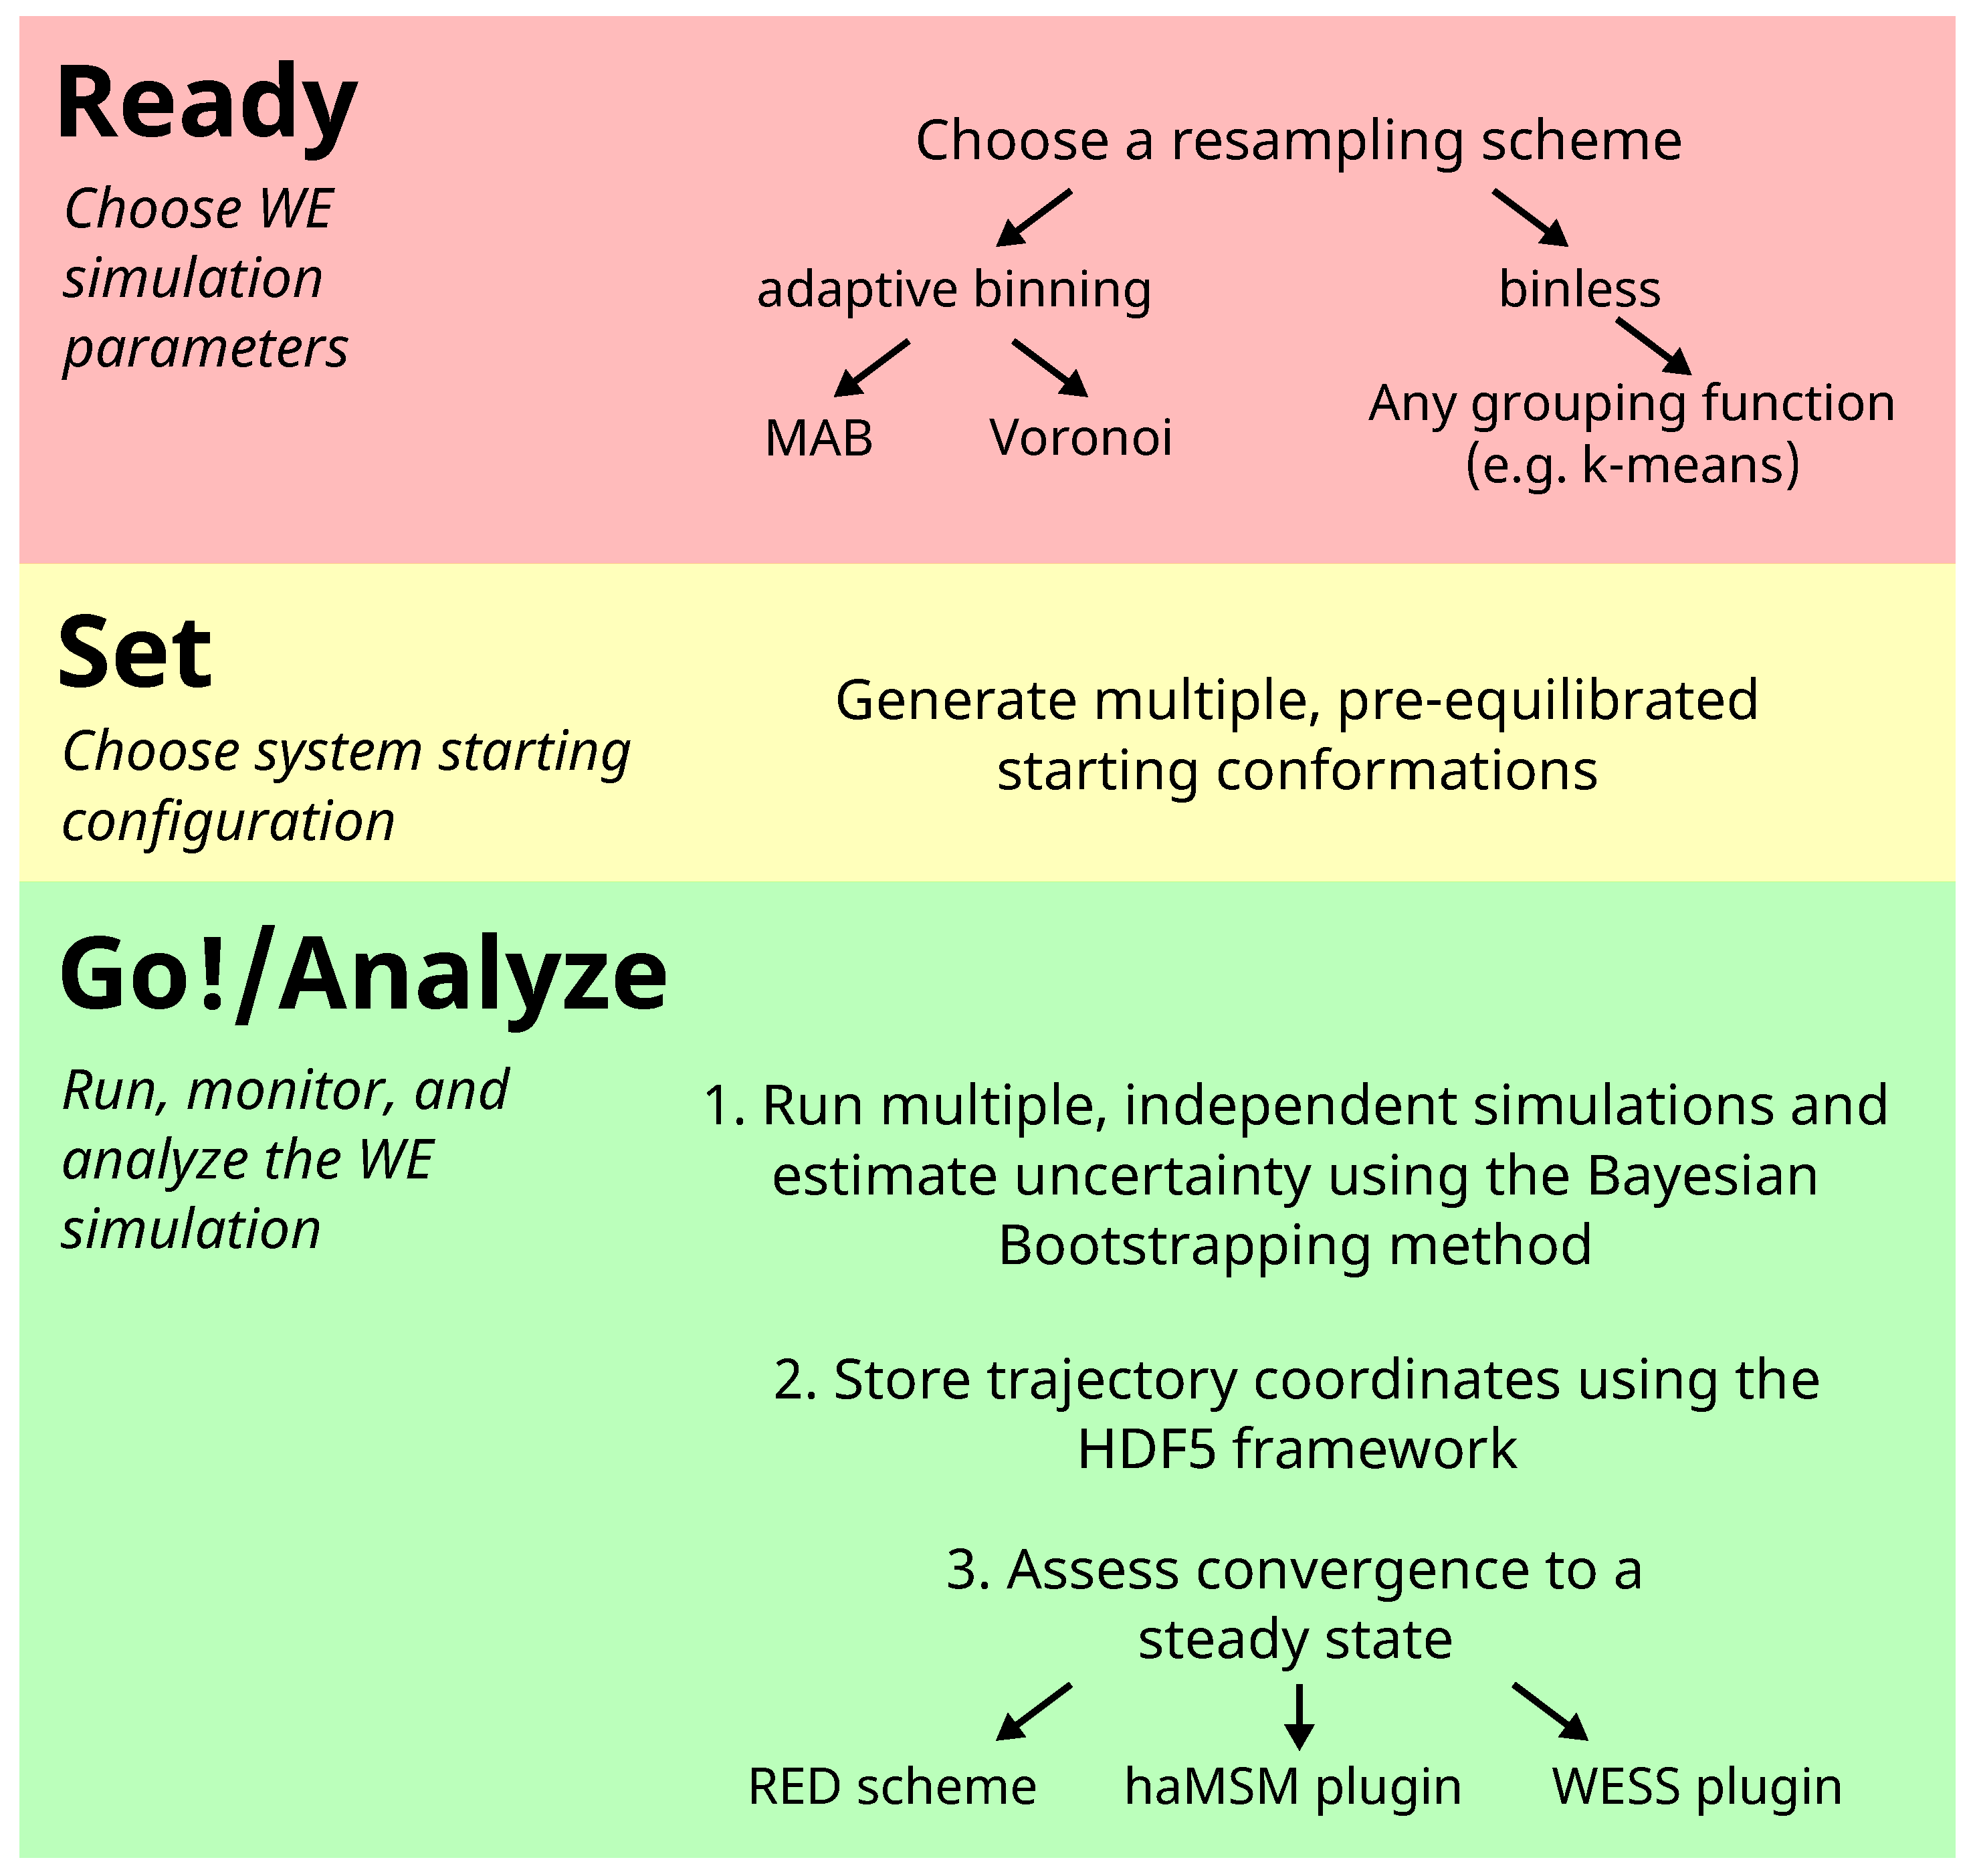
\includegraphics[width=\columnwidth]{figures/Figure2_workflow.pdf}
\caption{Recommended simulation workflow that makes use of major upgrades in the WESTPA 2.0 software.}
\label{fig:workflow}
\end{figure}

\section{General Guidelines for Choosing WE Parameters}
\label{intro:general-guidelines}
Suitable WE parameters such as the progress coordinate, binning scheme, and resampling interval $\tau$ depend on the particular system under investigation and the particular process of interest. 
Note that all of these WE parameters are tightly coupled to one another. Below are general recommendations that aim to assist in choosing these parameters. 
See Table 1 for examples from the literature. 
Currently, choosing WE parameters is something of an art, although the hope is to automate some aspects of parameter selection in the future. 
For now, we suggest what may be considered a semi-systematic, trial-and-error procedure:

\begin{enumerate}
\item Initially, choose the simplest 1D coordinate that would be expected to capture the slowest relevant motion along with initial bin spacings, $\tau$ value, and number of trajectories/bin. 
Choose these initial parameters following examples in the tutorials and/or literature, bearing in mind they likely will require modification.
\item The $\tau$ value should be sufficiently long such that at least one trajectory progresses to the next bin. 
In addition, a code scaling test (plot of the time required to complete a WE iteration vs. $\tau$ value) should be carried out for a range of potential $\tau$ values on the intended computer hardware to identify a $\tau$ value that yields reasonable linear scaling. 
\item If your system stops advancing along your progress coordinate, consider reducing the $\tau$ value, increasing the number of trajectories/bin, and/or using a finer bin spacing in that region of the progress coordinate while combining bins from higher probability regions. 
Note that bin spacings are arbitrary in WESTPA and the most efficient bin sizes likely are not exactly equal. 
Details for combining and creating bins “on-the-fly” are provided below in the \textbf{Intermediate Tutorial \ref{tut:p53-int}}. 
\item If none of the above efforts in step 3 are effective based on a one-dimensional progress coordinate, your progress coordinate may be missing orthogonal and relevant slow degrees of freedom. 
To address this issue, consider using a two-dimensional progress coordinate [\citep{Saglam2019,Zwier2016}; \textbf{Section \ref{tut:p53-int}}] or a “nested” coordinate in which the progress coordinate switches to monitoring another observable once a particular value for the initial observable is reached. 
Note that additional dimensions in the progress coordinate greatly increase the number of bins and hence the cost of the WE run, which is the motivation for nesting an additional coordinate in only a subset of the initial bins. 
You might also consider binning strategies that are not based on user-defined coordinates, but instead employ Voronoi cells potentially in conjunction with a string method. 
The WESTPA community will continue researching the important topic of self-adjusting adaptive bins. 
If all of your best efforts fail to generate transitions, consider simplifying your system (e.g. coarse-graining the model) and/or applying methods that involve the introduction of external forces (e.g. umbrella sampling) to generate initial transitions that can further inform the choice of progress coordinate.
\end{enumerate}

%%%
\begin{comment}
\subsection{Choosing WExplore-Specific Parameters}

WExplore is an algorithm that makes replicating and pruning decisions in a weighted ensemble framework.  We often call this a “resampler”.  WESTPA is a complete software package for running weighted ensemble simulations, including not only different resampling algorithms, but also scripts to setup, run and analyze weighted ensemble simulations.  Advanced Tutorial 2 shows how one can use the WExplore resampler inside the WESTPA toolkit. 

Regions in WExplore are hierarchically-organized Voronoi polyhedra, which are defined by a set of central points called “images” (\textbf{Figure \ref{fig:voronoi}}). 
To assign a trajectory to a given region, the distance from that trajectory to each image is measured, and the trajectory is assigned to the region with the lowest such distance. 
Key parameters in the WExplore method are the number of levels in the region hierarchy, the spacing between the images at each level of the hierarchy, the maximum branching factor of the hierarchy and the choice of distance metric. 
Each of these parameters is discussed below. 
In addition, factors affecting the optimal number of trajectories are discussed.

%%%Fig 2%%%
\begin{figure}
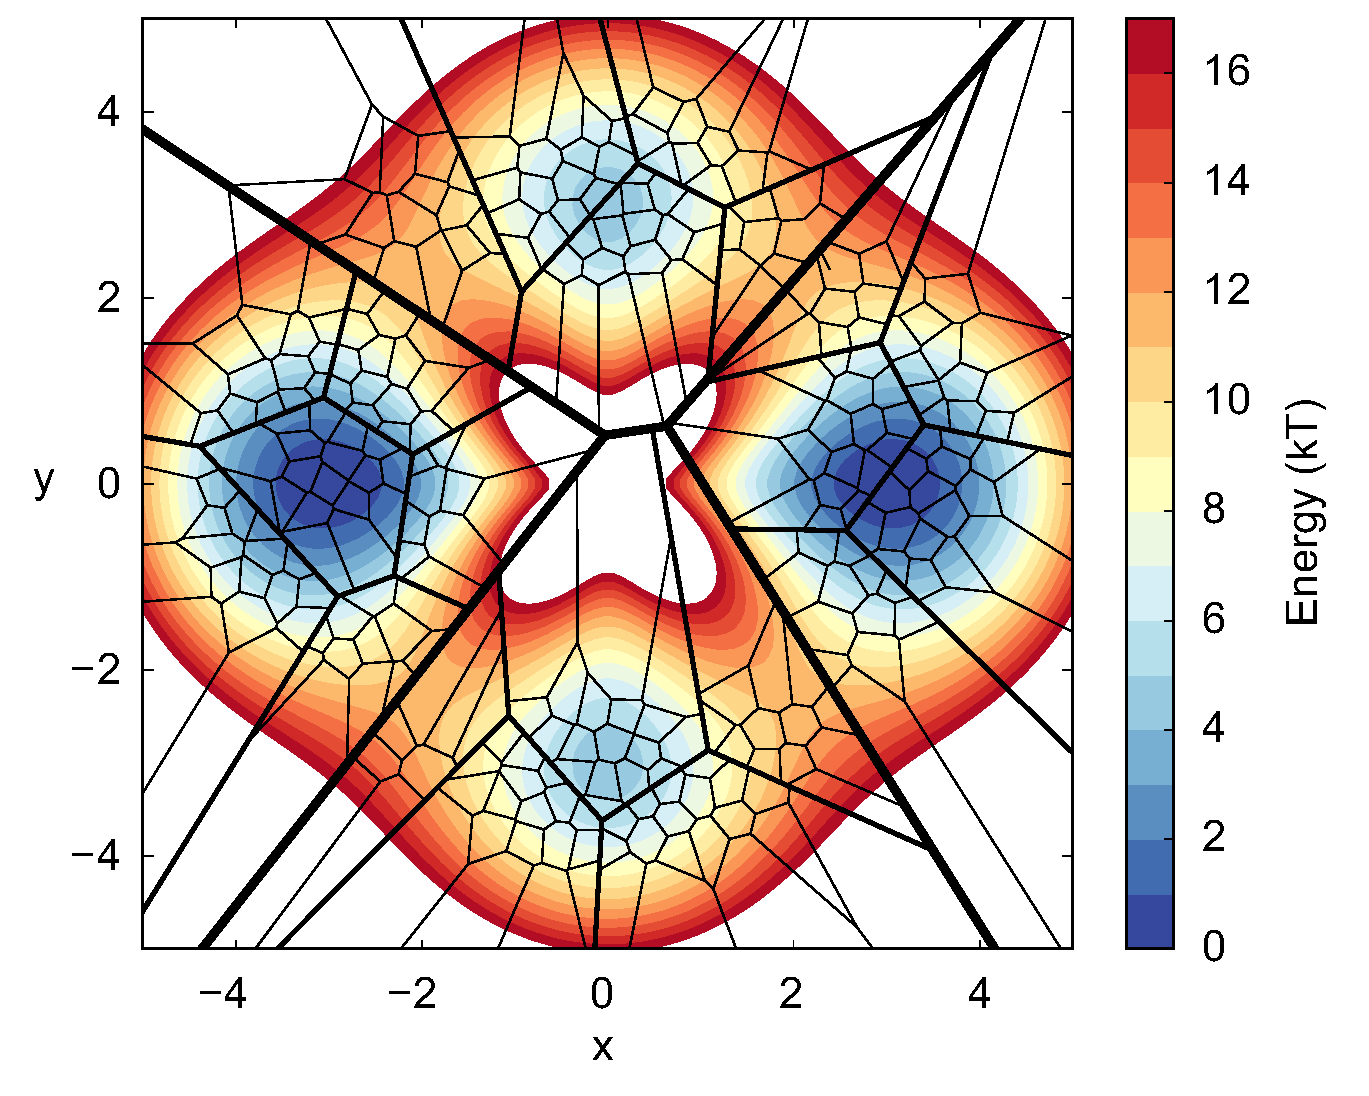
\includegraphics[width=\linewidth]{Figure2.eps}
\caption{Hierarchical Voronoi polyhedra for the ring potential model system \citep{Dickson2009,Adelman2013}.  
The blue colors show potential energy minima on the left and right and shallower minima on the top and bottom. 
Heavy lines show the Voronoi boundaries between the largest regions; one region is defined per local energy minimum.  
Each of these is broken up by medium regions (shown with medium-weight lines), which are themselves broken up by smaller regions (shown with light-weight lines).}
\label{fig:voronoi}
\end{figure}
%%%%%%%%

\textbf{Choice of Distance Metric.} Similar to the choice of progress coordinate in conventional WE, the distance metric used in WExplore should capture the slow degrees of freedom that are relevant to the process of interest. 
The distance metric could for instance be an RMSD (root mean squared distance) measurement, but focusing only on a subset of the system atoms. 
For instance, a common distance metric used in ligand (un)binding simulations is calculated by aligning binding site atoms, and calculating the RMSD between the ligands, without any further alignment \citep{Dickson2016}. 
Alternatively, a series of $N$ progress coordinates can be calculated as ${\bf X} = {\chi_1, \chi_2, \chi_3, …, \chi_N}$, and the Euclidean distance between two progress coordinate vectors can be used as the distance metric: $d_{ij} = |X_i - X_j|$. 
Many other examples are possible, and the researcher is only limited by their imagination. 
The distance used does not need to be differentiable or continuous.

\textbf{Region Size, Number of Levels, Branching Factor.} Once the distance metric is defined, the best practice is to run a short, straightforward simulation and observe the scale of fluctuations.
To be effective, the smallest region size (at the lowest level of the hierarchy) should be just outside the reach of the typical fluctuations observed in a time period $\tau$. 
This ensures that the first replication events will correspond to significant differences between trajectories. 
At the other end, the largest regions should be big enough that a set of $B$ regions can evenly tile the space of interest, where $B$ is the branching factor. 
Typically, $B$ is set to 10, which is low enough to offer a big efficiency boost in region assignment, and high enough that branch factor overflows (where the simulation attempts to create a region higher than the branch number) do not occur early on in the simulation. 
The optimal number of levels between the smallest and the largest region sizes is system dependent. 
If simulations are routinely getting stuck on one level for long time periods, this could indicate that the spacing between levels is too large. 
If simulations very easily proceed from one to the next then the spacing might be too small. 
It is difficult to know beforehand what the optimal spacing will be, but suitable parameters can be easily found using a little common sense and a bit of trial-and-error.

\textbf{Number of Trajectories.} In contrast to conventional WE, WExplore does not employ a fixed number of trajectories (N\textsubscript{t}) per region. 
This would be wildly impractical, as the typical total number of regions is very large (e.g. 10000 for a branching factor of 10 and a four-level hierarchy). 
Previous applications have aimed to choose N\textsubscript{t} to be as small as possible, while still allowing for simultaneous sampling of all states of interest, with a convenient value being 48, which is nicely congruent with 4-, 6- and 8-GPU compute servers \citep{Dickson2017,Dixon2018,Lotz2018}. 
A larger value will result in more consistent runs, while a smaller value allows for longer runs and more replicates. 
In practice we have found that single WExplore runs show high autocorrelation regardless of the value of N\textsubscript{t}, and that averaging over multiple replicates is a necessity, both to accurately compute observables and to estimate their uncertainty.

\end{comment}

\section{Cluster-Specific Considerations}

To take full advantage of WESTPA’s scaling and parallelizability, users may seek to run the software on HPC clusters.
The tutorials included herein are written with the goal of teaching new and relatively inexperienced users the basics of using the software and therefore do not focus on optimizations pertaining to the code. 
We recommend that users become familiar with running WESTPA on a cluster, especially the cluster-specific issues and considerations that may arise.

\subsection{Minimizing the Number of Output Files}
\label{intro:minimizing_traffic}
It is advisable to minimize the number of output files generated by your simulation as this reduces the I/O overhead and will therefore be less taxing on the filesystem of the computing cluster. 
We recommend saving only the restart files that are necessary for continuing trajectories and analysis of the simulation. 
If the user needs additional information (e.g. coordinates that have been saved at a greater frequency than the $\tau$ value) contained in certain output files, those files should of course be kept. 
To further reduce the number of files, we suggest separately tarring up the files for each WE iteration. 
The resulting tarballs will also facilitate any transferring of your simulation data to another location. 

In some cases such as WE simulations that are run using GPUs, trajectory segments can complete too quickly, leading to a bottleneck where the transfer of files over the network to the local storage of the node is too slow or there are too many transfers over the network. 
In such cases, copy over the data of the entire previous WE iteration as a tarball  to the local storage of the node, run the entire iteration from this local storage, and copy back the results to the scratch space in a single tarball. 
While these transfers over the network will add some overhead to each WE iteration, they will avoid the network bottleneck. 

\subsection{Data Management}

A single WE simulation may generate multiple terabytes of data, presenting a challenge for storage and retrieval of data. 
Moreover, using short trajectory segments in WE simulations commonly results in a large numbers of small files, which are managed more slowly on some file systems than a smaller number of large files with the same overall disk size. 
To alleviate these potential issues, we recommend the following:

\begin{enumerate}
\item Perform an initial run to monitor data storage and retrieval. 
Note that the initial number of trajectory segments may be a small fraction of the amount that would be generated in the eventual production run. 
\item Delete unnecessary files as each trajectory segment is simulated (see example \verb|runseg.sh| files in the \textbf{Basic and Intermediate Tutorials \ref{tut:nacl-basic}-\ref{tut:chig-int}}). 
Unnecessary files may include input files, log files from analysis tools, and raw text output files from analysis tools. 
Often, useful data from log files (e.g., temperature from an MD simulation) may be extracted from the log files and saved as auxiliary data to the WESTPA data file (\verb|west.h5| file), which stores data more efficiently than raw text.
\item Tar and optionally compress data from each WE iteration. 
This strikes a balance between excessive file count and excessive file size, either of which is typically sub-optimal for long term storage, especially on tape systems that may not guarantee the integrity of large files.
\item Consider saving coordinates for only the solute atoms of your system to an H5 file.
\end{enumerate}
\pagebreak

\subsection{Minimizing Network Traffic Across Multiple Computing Nodes}
Given the large scale of a WESTPA simulation, it is advisable to limit the number and frequency of network operations (e.g. I/O operations and file transfers from the local disk to the global filesystem). 
We recommend the following strategies for reducing network traffic:

\begin{enumerate}
\item Perform a code scaling test to identify an appropriate $\tau$ value (see \textbf{Section \ref{intro:general-guidelines}} above). 
\item Set environment variables to the full pathnames of repeatedly used programs (e.g. analysis tools used to calculate progress coordinates; see \textbf{Basic Tutorial \ref{tut:nacl-basic}}).  
\item Copy repeatedly accessed files (e.g. reference structures and analysis scripts) to local scratch space and temporarily write the output files to this scratch space. 
After each trajectory segment of length $\tau$ completes, tar the output files, and copy the tarred files to the globally accessible filesystem using \verb|rsync|. 
\end{enumerate}

\subsection{Advice when Using GPUs}

If your WE simulation has extremely frequent starting up of simulation segments, your simulation may overheat gaming GPUs and potentially damage the hardware. 
For example, folding simulations of the NTL9 protein in implicit solvent with a $\tau$ value of 15 ps resulted in such issues on gaming GPUs (i.e. NVIDIA GTX 1080Ti GPUs) while the same simulations have no such issues on professional-graphics-programming GPUs. 
Coarse-grained simulations (residue-level models and coarse-grained) with high I/O are also problematic on gaming GPUs. 

\section{Uncertainty Quantification and Monitoring of Convergence}

Although they can report on much longer timescales, WE calculations still have limitations analogous to those of conventional MD simulations -- namely, force field inaccuracy and inadequate sampling. 
Assessing convergence requires care, as noted below. 
Even if sampling is adequate, as with any simulation result, error bars are required to set the results in context because there is always a finite range of results which are predicted in any stochastic calculation \citep{Grossfield2019}. 
Error analysis is particularly challenging because WE results ultimately depend on a large number of trajectories which typically are significantly correlated with one another due to repeated replication (“splitting”) events. 
Over the years, different error analyses have been employed \citep{Zhang2007,Zwier2016,Mostofian2019}. 
Here we give a brief overview of current practice.

The primary recommendation is to perform multiple, fully independent WE simulations when possible.
To understand the variation intrinsic to WE sampling, we suggest performing these runs from identical starting states. 
The data from these runs will not go to waste, as it can be combined for estimating observables, convergence, and error bars. 
When multiple runs are not feasible for a large-scale application, a sufficiently large number of trajectories/bin (at least 4 trajectories/bin) should be used to increase the chances of obtaining a diverse ensemble of pathways. 
To further enhance the diversity of the pathways, we recommend starting the simulation from multiple starting states when that is physically appropriate such as in protein binding. 
We note that a single run with a large number of trajectories/bin (4-50 trajectories/bin) has been shown to be more efficient in calculating rate constants than multiple runs with a small number of trajectories/bin (i.e. < 4 trajectories/bin) for molecular association/dissociation systems \citep{Pratt2019}. 

We focus here on understanding uncertainty in rate-constant estimation. 
First, there is the issue of “convergence”: how much time is required to obtain a result without systematic bias that is governed only by statistical noise? 
In a typical simulation started in a single state (A), the rate constant into a target state B is estimated by the steady-state probability flux into B -- i.e., the amount of probability arriving per unit time as sketched in \textbf{Figure \ref{fig:converge}}. 
However, there is a transient regime before the flux levels off to its steady value, and it is unknown in advance how long the transient will last. 
Of course, one should examine the time-dependence of the average flux (averaged over all WE runs) by eye, but this is unlikely to be sufficient. 
In addition, one can plot the flux as a function of some continuous coordinate which progresses from A to B: in steady state, the flux will be constant along any such coordinate \citep{Jeremy2019}.
Finally, we recommend using a “history augmented” Markov state model (haMSM) employing very fine bins/microstates, which can be built from the WE data as a different means for estimating steady-state flux values which can be compared to those measured directly in WE simulation \citep{Jeremy2019}. 
Alternatively, the impact of transient effects on rate-constant estimation can be reduced by incorporating the distribution of event durations (excluding dwell time in the initial stable state) that correspond to pathways captured by the simulation. 
This strategy has been shown to yield rate constants using a fraction of the simulation time required by the original WE method \citep{DeGrave2019}. 

Once the transient has completed, if multiple runs were performed, it is necessary to estimate the uncertainty in the rate constant based on the group of independent WE runs. 
The flux curves from the individual runs, plotted as a function of molecular time, may vary significantly as sketched in Figure \ref{fig:converge}. 
This large variation invalidates typical uncertainty estimation schemes based on the standard error of the mean, and we therefore recommend employing a Bayesian bootstrapping procedure \citep{MostofianJCTC2019}. 
This approach appears to be better than alternative approaches for handling estimates which vary over orders of magnitude, but we emphasize that the nominal 95\% “credibility regions” produced are overly optimistic and only cover the true mean a much smaller percentage of the time \citep{MostofianJCTC2019}.

%%%Fig 3%%%
\begin{figure}
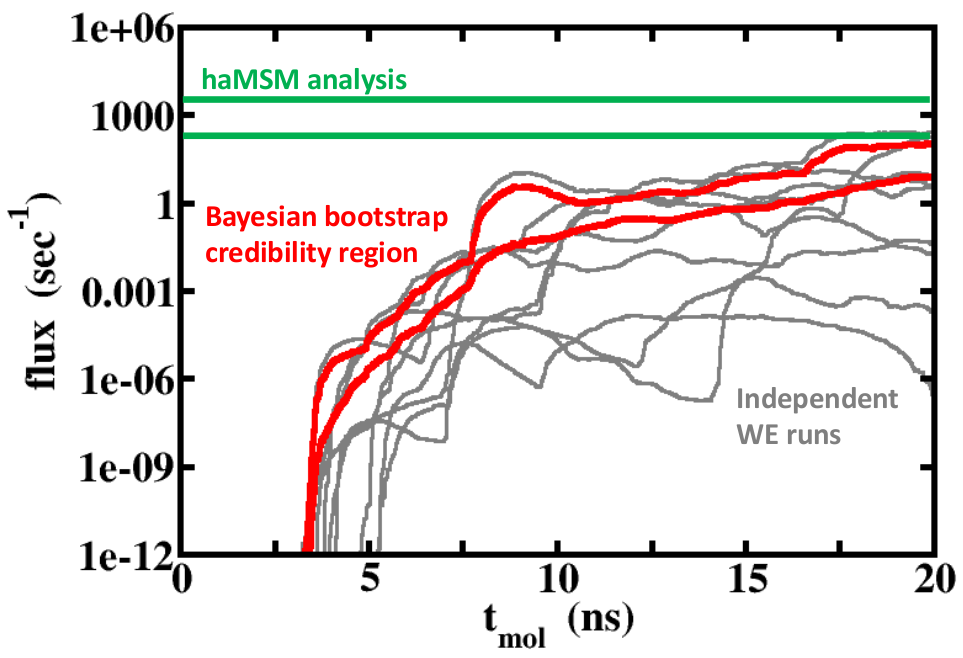
\includegraphics[width=\linewidth]{Figure3.png}
\caption{Convergence assessment and error analysis in the face of large run-to-run variation. 
The flux of probability into the target state B computed as a function of continuous molecular time, $t_{mol}$, is shown for several independent WE runs (grey). 
The large variation among individual runs makes it challenging both to assess whether the transient period has ended and to construct reliable error bars (see text). 
The history augmented Markov State Model (haMSM) analysis (green lines) provides an estimate of the long-time behavior, and the Bayesian bootstrap credibility region (red lines) estimates the average transient behavior.}
\label{fig:converge}
\end{figure}
%%%%%%%%


